\section{VHDL}
The VHDL code has been split up into small modules in order to heighten the level of abstraction, and to make it possible to reuse the code in other projects. 
The modules are as following; A top module that connects the different components, a module for serial communication with the ADC, a driver for the LED's, a PWM generator for the servo and a serial communicator to the PC using $\mu$TosNet.
\subsection{Top Module}
This module is only there in order to take the different components and put them together in order to make the application. This is done using components and port maps. A block diagram of the components used and how the internal signals are structured can be seen in figure \ref{fig::block_dia}.
\begin{figure}[h]
\centering
 \begin{tikzpicture}[node distance=4 cm]
 
 \node[module,minimum height= 5 cm,name=top] {TOP};
 \node[module,name=tosnet,right of = top] {$\mu$TosNet};
 \node[module,name=spi, above of = tosnet] {SPI};  
 \node[module,name=led_control, right of = spi] {LED\_driver};
 \node[module,name=motor,right of = tosnet] {Motor\_Control};
 \node[rectangle,minimum width = 2 cm, minimum height = 5 cm,name=empty, left of = top] {};
                      
 \draw[<-] (top.100) |- node[anchor=south]{\scriptsize MOSI}  (spi.150);
 \draw[->] (top.95)  |- node[anchor=south,xshift=0.5cm]{\scriptsize MISO} (spi.170);
 \draw[<-] (top.90)  |- node[anchor=south,xshift=1cm]{\scriptsize SCLK} (spi.190);
 \draw[<-] (top.85)  |- node[anchor=south,xshift=1 cm]{\scriptsize CS}   (spi.210);

 \draw[vecArrow] (top.122) to node[anchor=south]{\scriptsize LED[2:0]}  (empty.58);
 \draw[->] (top.135) to node[anchor=south]{\scriptsize pwm\_out}  (empty.45);
 \draw[->] (top.150) to node[anchor=south]{\scriptsize MOSI}  (empty.30);
 \draw[<-] (top.170) to node[anchor=south]{\scriptsize MISO} (empty.10);
 \draw[->] (top.190) to node[anchor=south]{\scriptsize SCLK} (empty.350);
 \draw[->] (top.210) to node[anchor=south]{\scriptsize CS}   (empty.330);
 \draw[->] (top.225) to node[anchor=south]{\scriptsize Serial Out}   (empty.315);
 \draw[<-] (top.235) to node[anchor=south]{\scriptsize Serial In}   (empty.305);
 
 \draw[vecArrow] (spi.40) to node[anchor=south]{\scriptsize Data\_out[9:0]} (led_control.140);
 \draw[vecArrow] (led_control.165) to node[anchor=south]{\scriptsize Data\_in[4:0]} (spi.15);
 \draw[<-] (spi.345) to node[anchor=south]{\scriptsize Data\_in\_ready} (led_control.195);
 \draw[->] (spi.325) to node[anchor=south]{\scriptsize Data\_out\_ready} (led_control.215);
 
 \draw[vecArrow] (led_control) to node[anchor=west]{\scriptsize Color[3:0]} (motor); 
 \draw[->] (tosnet.200) to node[anchor = south]{\scriptsize Serial Out} (top.340);
 \draw[->] (top.east) to node[anchor = south] {\scriptsize Serial in} (tosnet.west);
 \draw[->] (motor) |- node[anchor = south,xshift=-2 cm]{pwm\_out} (top.300);
 
 \draw[vecArrow] (tosnet.east) to ++(0.7,0) to ++(0,1.5) -| node[anchor=north,xshift=-0.7cm]{\scriptsize Threshold[31:0]} (led_control.240);
 \draw[vecArrow] (led_control.230) to ++(0,-0.7) -| node[anchor=south,xshift=1cm]{\scriptsize color\_val[31:0]} (tosnet.60);
 
 \end{tikzpicture}
 \caption{Block diagram of the system}
 \label{fig::block_dia}
\end{figure}


\subsection{LED\_driver}
This module is the brain of the project. This is where it is decided which LED should be on at the given moment, it takes the samples from the ADC, it analyzes the results of the ADC and decides which color the brick is.

\subsubsection{Implementation}
In order to make this work, a state machine is implemented. 
A state diagram of the system can be seen figure \ref{fig::state_led}. 
It starts in in red state. 
In this state the red LED is turned on, and a sample from the ADC is done. 
To make make the system stable to step responses, the two first ADC readouts are thrown away.
This is discussed further in section \ref{sec:rise_time_test}.
After the third readout from the ADC, the state is changed and the other LED's are flashed one at a time, and the value of the photo diode is read from the ADC. 
The last state is the decider state which interprets the values and decides what color the brick is.
It is shown in section \ref{sec:system_test} that just looking at the highest value is not good enough for classification.
Instead, a nearest neighbor approach is used.
This means that each block is compared to all values.
Ideally a red block would reflect a lot of red light and small amounts of green and blue light.
So instead of going with the highest value, this method looks at an approximation of the distance between the current measurements and the ideal block.
This is usually done by comparing euclidean distances, but this has been simplified to the sum of the absolute difference.
The block values can be updated from the computer through $\mu$TosNet. 

\begin{figure}[h]
\centering
 \begin{tikzpicture}[node distance=2.5cm]
 
 \node[circle,minimum width = 7 cm,name = c]{};
%  \node[accepting,state,	name=state0, minimum width = 1.3 cm] at (c.90)    {Idle}; 
 \node[state,name=stateR, minimum width = 1.3 cm]            at (c.18)    {Red};
 \node[square,name=start,above of = stateR,yshift=-1.2 cm]                {Start};
 \node[state,name=stateG, minimum width = 1.3 cm]            at (c.-56)   {Green};
 \node[state,name=stateB, minimum width = 1.3 cm]            at (c.234)   {Blue};
 \node[state,name=decide, minimum width = 1.3 cm]            at (c.162)   {Decider};
 
%  \draw[->] (state0)   edge[bend left=27] node[midway,above,fill=white,xshift=0.9cm,yshift=-0.5cm] {ADC data $>$ threshold}  (stateR);
 \draw[->] (stateR)   edge[bend left=27] node[midway,fill=white]                                  {dummy\_count $=$ 2}      (stateG);
 \draw[->] (stateG)   edge[bend left=27] node[midway,below]                                       {dummy\_count $=$ 2}      (stateB);
 \draw[->] (stateB)   edge[bend left=27] node[midway,fill=white]                                  {dummy\_count $=$ 2}      (decide);
%  \draw[->] (decide)   edge[bend left=27] node[midway,below,fill=white]                            {sample\_count $=$ 4}     (state0);
 \draw[->] (decide)   to                 node[midway,above]                                       {}    (stateR);
 \draw[->] (start)    to                                                                                                    (stateR);
 
 \end{tikzpicture}
 \caption{State machine of \textbf{LED\_driver}}
 \label{fig::state_led}
\end{figure}

\subsubsection{Test of Decision State.}\label{sec:system_test}
To find the classifier values for the blocks, a test with a each color block and a test without any blocks were made.
This showed that the light intensities are not ideal and green and blue light gets reflected more than expected.
This should be compensated by the Nearest Neighbor approach.

The signal has been analyzed and the binary value corresponding to the tested ADC reading has been found for each block.
These numbers are then used in the code as the default values for each brick.
The numbers can be updated over the $\mu$TosNet protocol.

A c++ program has been made, which samples the ADC values and sets the classifier as the mean of the samples.

\subsubsection{Extra considerations}
One of the things that was thought of during implementation the Nearest Neighbor algorithm was whether or not there was logic enough in order to contain all of the data needed without using external memory. In the beginning a simpler algorithm was implemented, that uses thresholds in order to decide which color brick there is.
Finding the distances does not require the knowledge of the other colors, so they could all be implemented concurrently if they are run in the same clock cycle in a process.
This was tested to use 98\% of the slices on the board.
Instead, each color was handled at separate clocks, to allow for modules to be reused by the place and route application.
This got the utilization down to 86\%.
Another drawback of running everything in a single process is clock skew.
If not specified, Xilinx does not know the clock speed of the device.
Thus it will warn the user about potential clock skew.
If the skew gets above the period, the FPGA cannot be ready to run the process again and the behavior gets unpredictable.
The current clock skew with the nearest neighbor approach is $14.316 ns$, which is in a dangerous zone, but below the threshold. 

\begin{figure}[H]
 \centering
\setlength{\belowcaptionskip}{5pt}

\begin{subfigure}[b]{0.70\textwidth}
\centering
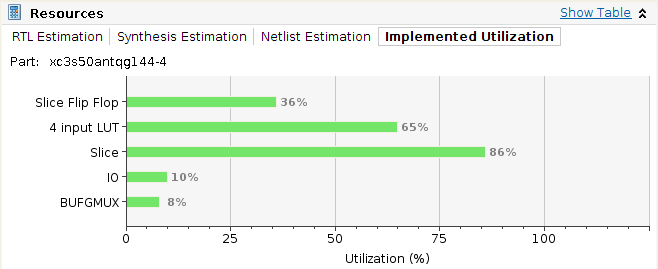
\includegraphics[width=\linewidth]{img/nearest_neighbor_optimized.png}
\caption{Logic consumption of the project with Nearest Neighbor algorithm as decider.}
\end{subfigure}

\begin{subfigure}[b]{0.70\textwidth}
\centering
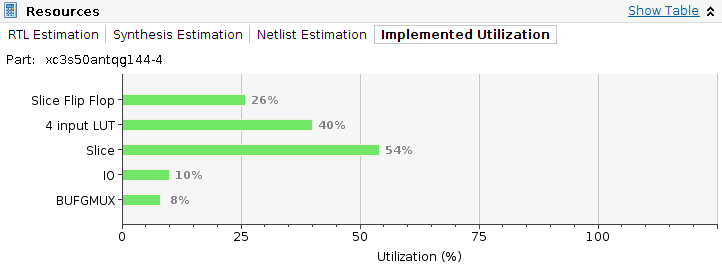
\includegraphics[width=\linewidth]{img/thresholding.png}
\caption{Logic consumption of project with a simple thresholding algorithm as decider.}
\end{subfigure}

\end{figure}

\subsection{SPI}
The analog to digital converter (ADC) supplied by the supervisor uses a SPI protocol as it's form of communication, so a module in the FPGA needs to be set up.

\subsubsection{Protocol}
The FPGA will serve as the master and the ADC as the slave. In the VHDL module a clock is generated in order for the slave to have a signal on which to send data out, making the communication synchronous. The communication is full-duplex, and the master puts data out on it's wire (MOSI) before the falling edge of the serial clock, in order for the ADC to read it, which is done on the falling edge. The reverse is happening on the slave. It puts data out on it's wire (MISO) before the rising edge of the serial clock for the master to read on rising edge. The ADC does not sample continuously, but it has to be requested data. A request can be seen in figure \ref{time_spi_sample}. What is happening is that the master putting chip select (CS) low, and it sends a command to the ADC. The content of the command is a start bit, a configuration bit, which tells the ADC if it is running single or differential mode and 3 bits to select the channel. After this the status of the MOSI is \textit{don't care}. In order for the ADC to make the sample and hold, it needs the time of one clock cycle in order for the internal capacitor to charge, so after the last bit of the channel one clock cycle, nothing happens. After this cycle the data is clocked out. When the master has received 10 bits of data, CS is taken high and the clock is shut off.

\begin{figure}[h]
 \centering
 \begin{tikztimingtable}
  CLK	& H35{T}H\\
  CS	& H35{L}H\\
  MOSI	& LL2D{S}2D{S/D}6D{CH}25{U}\\
  MISO	& 14{Z}22D{ADC DATA}Z\\
 \end{tikztimingtable}
\caption{Timing diagram of taking one sample}
\label{time_spi_sample}
\end{figure}

\subsubsection{Implementation}
Given the datasheet\cite[p. 1]{ds:MCP3008},
the maximum clock frequency of the SPI clock is $3.6$ MHz which gives a period time of 277 ns. 
This is not possible to obtain due to the system clock period being 20 ns. 
This is rounded to 280, which divides evenly with 20 and gives a clock frequency of $3.571$ MHz. 
Therefore a clock is generated with this period time in this VHDL module and put out on an output pin.

In order to keep the abstraction level, that this module is only for communication, it is the {LED\_driver} module that tells the {spi\_module} to initiate a sample. 
When a sample is received the data is just passed on to the LED\_driver, and a flag is set in order to tell the driver that new data has arrived.

\subsection{MotorControl}
In order to make the sorting happen, a servo motor with a mounted plastic rod is used. The colors that the {LED\_driver} has detected is fed in to the module, one wire for each color. The motor controller then decides which way the rod should point. If there are more than one color wire that is high, the rod is placed in the middle. 

The servo motor is controlled by a pulse width modulated (PWM) signal. The standard for RC-servo motors\cite[p. 917]{book:prac_ele}, one of which was provided for this project, a pulse width of 1 ms to be on the left extreme and 2 ms for the right extreme, with a PWM period of 20 ms. 
The pulse width for a desired angle can be calculated using equation \ref{eq:pulse_width}.
Here the max value of the motor has to be found.
The given motor has a max angle of 120 degrees but motors with 220 degrees exist.
Since it is not needed to go to the extremes, new width values has to be put in. 

\begin{equation}
 \text{pulse}_\text{width} = \frac{\text{desired}_{\text{angle}}}{\text{max}_{\text{angle}}}+\text{pulse}_{\text{normal}} \label{eq:pulse_width}
\end{equation}

The plastic rod has been measured to be $10 cm$ long and the rod should move $2.5 cm$ in either direction from the middle position.
Thus an angle of $14$ degrees is desired in both directions.
It was found out that these values should be $1.38 ms$ to make the bricks slide right and $1.62 ms$ to make them slide left.
With a $400$ division this means the pulse width should be $27.6$ clock cycles to make the rod go right and $32.3$ clocks to make it go to the left.
This was decided to be rounded towards maximum spread, thus choosing $27$ and $33$ clock cycles.
In figure \ref{fig:pwm_simulation} can the simulation of the pwm signal be seen.
The motor reacts on the color of the Lego and the different widths can be seen.

\begin{figure}[h]
\centering
    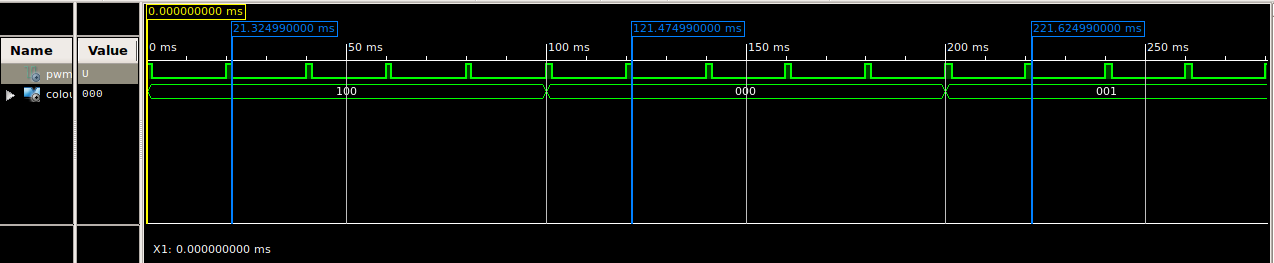
\includegraphics[width=0.9\linewidth]{img/pwm_simulation}
    \caption{Simulation of the pwm signal that controls the servo motor.}
    \label{fig:pwm_simulation}
\end{figure}

\subsection{$\mu$TosNet}
When working with an FPGA, especially with one with limited I/O pins, setting up some sort of user interaction is very limited and sometimes very primitive. This can be a problem if the system is complex. Therefore setting up communication with a PC could be a desired feature. A communication module called $\mu$TosNet is available and used. $\mu$TosNet uses UART, which is a serial communication using only 2 wires. This makes it good for non I/O heavy FPGA. 

\subsubsection{Usage}
Due to the process of compiling the bit file from VHDL is slow and tedious, it could be nice to be able to calibrate the different color classification from the computer instead of compiling and flashing every time you want to fine tune the system. This can be done for each color individually or a live calibration, with instructions.

To make the communication on the computer a small C++ program was made, using the Boost library to instantiate the serial communication, building on a skeleton found on the internet\cite{url:serial}.

The communication protocol is shown in figure \ref{fig:read_protocol}. 10 bits are used for each color and a control signal is sent in the remainding bits. %The ctrl bits shows which color is being guessed as the likely color.
The sending protocol is identical. Only this is used to overwrite the thresholds and the ctrl bits are used to specify which brick values are being overwritten.


\begin{figure}[h]
\centering
    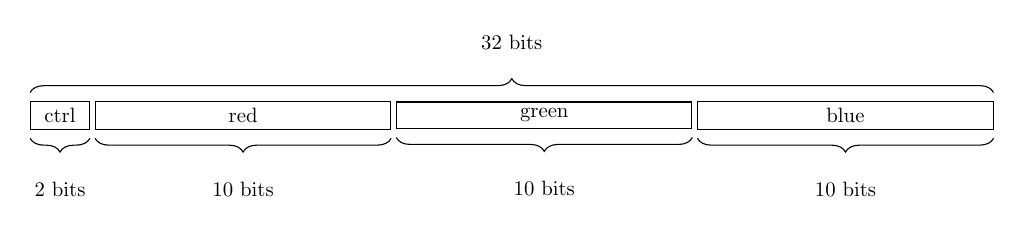
\begin{tikzpicture}[scale=0.75, every node/.style={scale=0.75}]
        \node[draw, color=black,text centered, minimum height=12pt, name=ctrl,   minimum width=1cm] at (0,0)                     {ctrl};
        \node[draw, color=black,text centered, minimum height=12pt, name=red,    minimum width=5cm,  right of=ctrl,   xshift=2.1cm] {red};
        \node[draw, color=black,text centered, minimum height=12pt, name=green,  minimum width=5cm,  right of=red,   xshift=4.1cm] {green};
        \node[draw, color=black,text centered, minimum height=12pt, name=blue,   minimum width=5cm,  right of=green,   xshift=4.1cm] {blue};
        
        \draw[decorate,decoration={brace,amplitude=5pt,raise=3pt}] (ctrl.north west) -- (blue.north east) node[midway,yshift=1cm] {32 bits} ;
        
        \draw[decorate,decoration={brace,amplitude=5pt,mirror,raise=3pt}] (ctrl.south west) -- (ctrl.south east) node[midway,yshift=-1cm] {2 bits} ;
        
        \draw[decorate,decoration={brace,amplitude=5pt,mirror,raise=3pt}] (red.south west) -- (red.south east) node[midway,yshift=-1cm] {10 bits} ;
        \draw[decorate,decoration={brace,amplitude=5pt,mirror,raise=3pt}] (green.south west) -- (green.south east) node[midway,yshift=-1cm] {10 bits} ;
        \draw[decorate,decoration={brace,amplitude=5pt,mirror,raise=3pt}] (blue.south west) -- (blue.south east) node[midway,yshift=-1cm] {10 bits} ;
    \end{tikzpicture}
    \caption[$\mu$tosnet data protocol.]{The data format used when sending data to and from the FPGA.}
    \label{fig:read_protocol}
\end{figure}
